\documentclass[aspectratio=169,12pt]{beamer}

% --- Modern theme setup ---
\usetheme{metropolis}
\setbeamertemplate{navigation symbols}{}
\setbeamercolor{frametitle}{bg=black!85, fg=white}
\setbeamercolor{progress bar}{fg=orange!80!black}
\setbeamercolor{alerted text}{fg=orange!80!black}

\usepackage[utf8]{inputenc}
\usepackage[T1]{fontenc}
\usepackage{amsmath,amssymb}
\usepackage{graphicx}
\usepackage{booktabs}
\usepackage{multirow}
\usepackage{tikz}
\usetikzlibrary{shapes,arrows.meta,positioning,fit,calc,decorations.pathreplacing}
\usepackage{xcolor}
\usepackage{fontawesome5}
\usepackage[normalem]{ulem}

% Custom colors
\definecolor{hhi}{RGB}{0, 82, 136}
\definecolor{accent}{RGB}{230, 126, 34}
\definecolor{success}{RGB}{39, 174, 96}
\definecolor{danger}{RGB}{231, 76, 60}
\definecolor{muted}{RGB}{127, 140, 141}

\title{Health-Aware Block Scheduling\\for LNG Carrier Production}
\subtitle{ISE 572 --- Reinforcement Learning Meets Shipbuilding}
\author{Stephen Eacuello \and Steven Blum}
\date{Spring 2026}
\institute{University of Rhode Island}

\begin{document}

%==============================================================
% TITLE
%==============================================================
\begin{frame}
\titlepage
\end{frame}

%==============================================================
\section{The Problem}
%==============================================================

%--------------------------------------------------------------
% SLIDE: Hook
%--------------------------------------------------------------
\begin{frame}{A \$200M Scheduling Problem}

\begin{columns}[T]
\column{0.55\textwidth}

\vspace{0.5em}
An LNG carrier costs \textbf{\$200M+} and takes \textbf{2--3 years} to build.

\vspace{1em}
Each ship is assembled from \textbf{200 blocks}, each passing through \textbf{8 production stages}, moved by \textbf{24 transporters} and lifted by \textbf{9 cranes}.

\vspace{1em}
Today, this scheduling is done \textbf{manually} --- by experienced planners using spreadsheets and intuition.

\vspace{1em}
{\color{accent}\textbf{Question:}} Can we learn a policy that schedules better than a human expert?

\column{0.42\textwidth}

\includegraphics[width=\textwidth]{figures/shipyard_layout.png}

\vspace{0.3em}
{\footnotesize\color{muted} HD Hyundai Heavy Industries\\Ulsan, South Korea\\World's largest shipyard}
\end{columns}
\end{frame}

%--------------------------------------------------------------
% SLIDE: Contributions
%--------------------------------------------------------------
\begin{frame}{What We Did}

\begin{enumerate}
    \setlength\itemsep{1em}
    \item \textbf{Built a full simulation} of HHI Ulsan --- 200 blocks, 10 docks, 9 cranes, 24 SPMTs, with NSRP-calibrated processing times
    \item \textbf{Discovered entropy collapse} --- PPO/SAC fail catastrophically in hierarchical masked action spaces (entropy $\to$ 0 by epoch 5)
    \item \textbf{Solved it with DAgger} --- imitation learning achieves \textbf{97.0\% $\pm$ 2.5\%} of expert (10-seed validation), bypassing the exploration problem entirely
    \item \textbf{Exposed a scalability wall} --- all methods (RL, OR, imitation) fail to scale beyond 200 blocks; simple EDD dispatch remains king at scale
\end{enumerate}
\end{frame}

%--------------------------------------------------------------
% SLIDE: Production pipeline (visual, minimal text)
%--------------------------------------------------------------
\begin{frame}{How a Ship Gets Built}
\centering
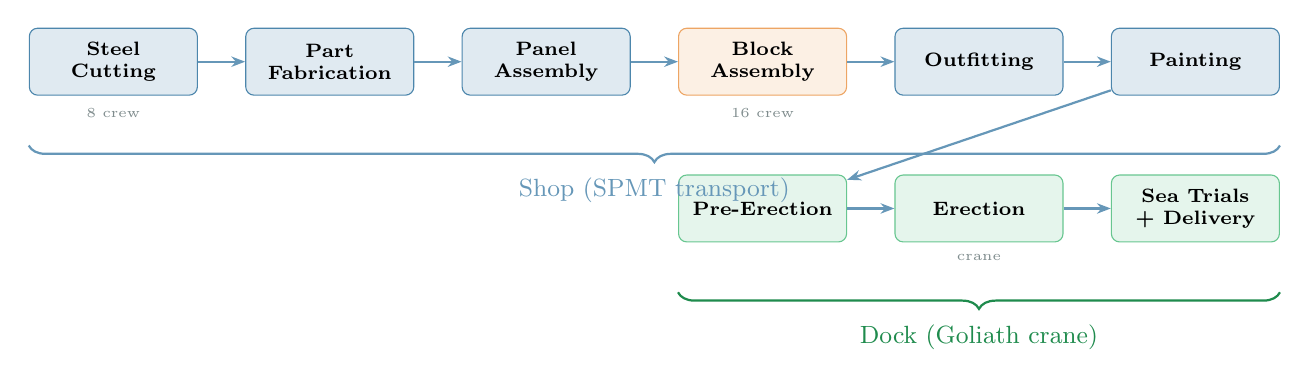
\begin{tikzpicture}[
    node distance=0.6cm,
    stage/.style={rectangle, rounded corners=3pt, draw=#1!70, fill=#1!12,
                  text width=1.9cm, minimum height=0.85cm, align=center,
                  font=\scriptsize\bfseries},
    stage/.default=hhi,
    arrow/.style={-{Stealth[length=5pt]}, thick, hhi!60},
    label/.style={font=\tiny\color{muted}, below=1pt}
]
% Row 1: Shop stages
\node[stage=hhi] (s0) {Steel\\Cutting};
\node[stage=hhi, right=of s0] (s1) {Part\\Fabrication};
\node[stage=hhi, right=of s1] (s2) {Panel\\Assembly};
\node[stage=accent, right=of s2] (s3) {Block\\Assembly};
\node[stage=hhi, right=of s3] (s4) {Outfitting};
\node[stage=hhi, right=of s4] (s5) {Painting};

% Row 2: Dock stages
\node[stage=success, below=1cm of s3] (s6) {Pre-Erection};
\node[stage=success, right=of s6] (s7) {Erection};
\node[stage=success, right=of s7] (s8) {Sea Trials\\+ Delivery};

% Labels
\node[label] at (s0.south) {8 crew};
\node[label] at (s3.south) {16 crew};
\node[label] at (s7.south) {crane};

% Arrows
\draw[arrow] (s0) -- (s1);
\draw[arrow] (s1) -- (s2);
\draw[arrow] (s2) -- (s3);
\draw[arrow] (s3) -- (s4);
\draw[arrow] (s4) -- (s5);
\draw[arrow] (s5) -- (s6);
\draw[arrow] (s6) -- (s7);
\draw[arrow] (s7) -- (s8);

% Braces
\draw[decorate, decoration={brace, amplitude=6pt, mirror}, thick, hhi!60]
    ([yshift=-18pt]s0.south west) -- ([yshift=-18pt]s5.south east)
    node[midway, below=8pt, font=\small] {Shop (SPMT transport)};
\draw[decorate, decoration={brace, amplitude=6pt, mirror}, thick, success!80!black]
    ([yshift=-18pt]s6.south west) -- ([yshift=-18pt]s8.south east)
    node[midway, below=8pt, font=\small] {Dock (Goliath crane)};
\end{tikzpicture}

\vspace{1em}
\begin{columns}[c]
\column{0.3\textwidth}\centering
{\Large\color{hhi}\textbf{200}} blocks/ship
\column{0.3\textwidth}\centering
{\Large\color{accent}\textbf{1.24M}} man-hours/ship
\column{0.3\textwidth}\centering
{\Large\color{success}\textbf{8}} production stages
\end{columns}
\end{frame}

%==============================================================
\section{Method}
%==============================================================

%--------------------------------------------------------------
% SLIDE: MDP (cleaner two-column)
%--------------------------------------------------------------
\begin{frame}{Formulation: Scheduling as an MDP}

\begin{columns}[T]
\column{0.48\textwidth}

\textbf{State}: Heterogeneous graph
\vspace{0.3em}
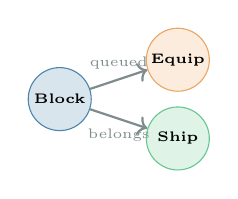
\begin{tikzpicture}[
    n/.style={circle, draw=#1!70, fill=#1!15, minimum size=8mm,
              font=\tiny\bfseries, inner sep=0pt},
    n/.default=hhi
]
\node[n=hhi] (b) at (0,0) {Block};
\node[n=accent] (e) at (1.5,0.5) {Equip};
\node[n=success] (s) at (1.5,-0.5) {Ship};
\draw[->, thick, muted] (b) -- node[above, font=\tiny] {queued} (e);
\draw[->, thick, muted] (b) -- node[below, font=\tiny] {belongs} (s);
\end{tikzpicture}

\vspace{0.5em}
GATv2 encoder $\to$ fixed $\mathbb{R}^{256}$ embedding\\
{\small\color{muted} Works for any number of blocks}

\column{0.48\textwidth}

\textbf{Action}: Hierarchical (10 heads)
\vspace{0.3em}

\begin{tabular}{@{}ll@{}}
{\color{accent}\faArrowRight} & \textit{What?} transport / erect / hold \\
{\color{accent}\faTruck} & \textit{Which SPMT?} (1 of 24) \\
{\color{accent}\faCube} & \textit{Which block?} (1 of 200) \\
{\color{accent}\faIndustry} & \textit{Which crane?} (1 of 9)
\end{tabular}

\vspace{0.8em}
\textbf{Reward}: $+1$ stage advance, $+10$ ship delivery, $-0.5$ per tardy step

\end{columns}

\vspace{0.5em}
\centering
{\small\color{muted} Action masking ensures only valid actions are sampled --- but this creates a problem\ldots}
\end{frame}

%--------------------------------------------------------------
% SLIDE: The Problem --- Entropy Collapse (the tension)
%--------------------------------------------------------------
\begin{frame}{The Core Problem: Entropy Collapse}

\begin{columns}[T]
\column{0.48\textwidth}

\includegraphics[width=\textwidth]{figures/entropy_collapse.png}

\column{0.48\textwidth}
\vspace{1em}
PPO entropy: \textbf{2.27 $\to$ 0.00} by epoch 5.

\vspace{0.5em}
The policy becomes \textit{completely deterministic} before it has learned anything useful.

\vspace{1em}
\textbf{Why?} Action masking reduces valid options to 1--2 choices. Entropy is \textit{mathematically bounded} by $\log k$, where $k$ is the number of valid actions.

\vspace{1em}
\textbf{Result:}\\
PPO: \textbf{0.4\%} of expert\\
SAC: \textbf{28.7\%} of expert\\
{\color{danger} Neither is usable.}
\end{columns}
\end{frame}

%--------------------------------------------------------------
% SLIDE: Our Solution --- DAgger
%--------------------------------------------------------------
\begin{frame}{Our Solution: Learn from an Expert via DAgger}

\begin{columns}[T]
\column{0.55\textwidth}

\includegraphics[width=\textwidth]{figures/curriculum_dagger.png}

\column{0.42\textwidth}
\vspace{0.5em}
\textbf{DAgger} (Dataset Aggregation):\\
Supervised learning from expert demonstrations --- no exploration needed.

\vspace{0.8em}
\textbf{Curriculum}: 3 stages
\begin{enumerate}
    \item Tiny: 10 blocks
    \item Small: 50 blocks
    \item Medium: 200 blocks
\end{enumerate}

\vspace{0.5em}
Each stage: $\beta$ anneals $0.8 \to 0.2$\\
{\small (expert $\to$ student control)}

\vspace{0.8em}
{\color{success}\textbf{Small instance: 97.0\% $\pm$ 2.5\% of expert}}\\
{\small 10-seed validation; best config reaches 100.5\% via error recovery}
\end{columns}
\end{frame}

%--------------------------------------------------------------
% SLIDE: Architecture (cleaner)
%--------------------------------------------------------------
\begin{frame}{Architecture}
\centering
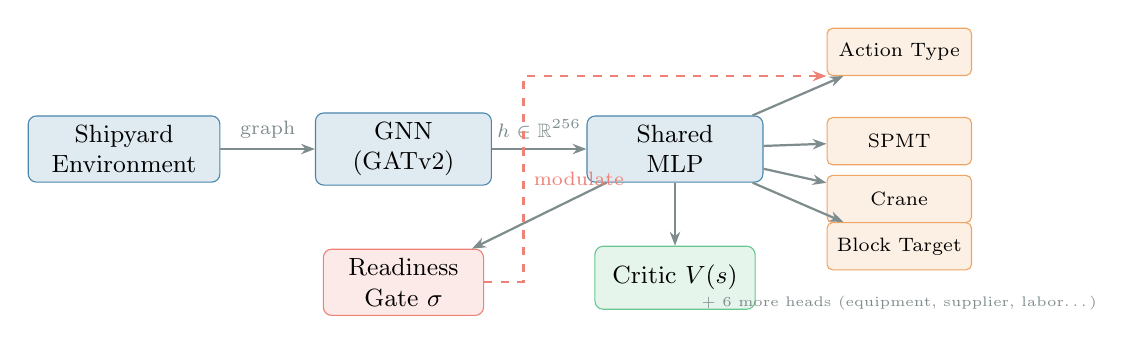
\begin{tikzpicture}[
    node distance=0.6cm,
    comp/.style={rectangle, rounded corners=3pt, draw=#1!70, fill=#1!12,
                 minimum height=0.8cm, align=center, font=\small},
    comp/.default=hhi,
    head/.style={rectangle, rounded corners=2pt, draw=accent!70, fill=accent!12,
                 minimum height=0.6cm, align=center, font=\scriptsize},
    arr/.style={-{Stealth[length=5pt]}, thick, muted}
]
% Main pipeline
\node[comp=hhi, text width=2.2cm] (env) {Shipyard\\Environment};
\node[comp=hhi, text width=2cm, right=1.2cm of env] (gnn) {GNN\\(GATv2)};
\node[comp=hhi, text width=2cm, right=1.2cm of gnn] (mlp) {Shared\\MLP};

% Heads fanning out
\node[head, text width=1.6cm, above right=0.5cm and 0.8cm of mlp] (h1) {Action Type};
\node[head, text width=1.6cm, right=0.8cm of mlp, yshift=0.1cm] (h2) {SPMT};
\node[head, text width=1.6cm, below right=-0.1cm and 0.8cm of mlp] (h3) {Crane};
\node[head, text width=1.6cm, below right=0.5cm and 0.8cm of mlp] (h4) {Block Target};

% Critic & Gate
\node[comp=success, text width=1.8cm, below=0.8cm of mlp] (critic) {Critic $V(s)$};
\node[comp=danger, text width=1.8cm, below=0.8cm of gnn] (gate) {Readiness\\Gate $\sigma$};

% Arrows
\draw[arr] (env) -- node[above, font=\scriptsize\color{muted}] {graph} (gnn);
\draw[arr] (gnn) -- node[above, font=\scriptsize\color{muted}] {$h \in \mathbb{R}^{256}$} (mlp);
\draw[arr] (mlp) -- (h1);
\draw[arr] (mlp) -- (h2);
\draw[arr] (mlp) -- (h3);
\draw[arr] (mlp) -- (h4);
\draw[arr] (mlp) -- (critic);
\draw[arr] (mlp) -- (gate);
\draw[arr, dashed, danger!70] (gate.east) -- ++(0.5,0) |- (h1.south west)
    node[pos=0.25, right, font=\scriptsize\color{danger}] {modulate};

% Label
\node[font=\tiny\color{muted}, below=0.2cm of h4] {+ 6 more heads (equipment, supplier, labor\ldots)};
\end{tikzpicture}

\vspace{0.5em}
\begin{columns}[c]
\column{0.3\textwidth}\centering
{\small\textbf{Readiness gate}\\logistic regression\\modulates dispatch}
\column{0.3\textwidth}\centering
{\small\textbf{10 action heads}\\only relevant heads\\contribute to $\log\pi$}
\column{0.3\textwidth}\centering
{\small\textbf{Action masking}\\invalid $\to$ $-20$ logits\\(soft, not $-\infty$)}
\end{columns}
\end{frame}

%==============================================================
\section{Results}
%==============================================================

%--------------------------------------------------------------
% SLIDE: The good news
%--------------------------------------------------------------
\begin{frame}{Result 1: DAgger Beats the Expert (on Small Instances)}

\begin{columns}[T]
\column{0.48\textwidth}

\includegraphics[width=\textwidth]{figures/method_comparison.png}

\column{0.48\textwidth}
\vspace{1em}
\begin{tabular}{@{}lrl@{}}
\toprule
\textbf{Method} & \textbf{vs Expert} & \\
\midrule
PPO & 0.4\% & {\color{danger}\faTimesCircle} \\
SAC & 28.7\% & {\color{danger}\faTimesCircle} \\
BC & 85.2\% & {\color{muted}\faMinusCircle} \\
GAIL & 78.4\% & {\color{muted}\faMinusCircle} \\
\textbf{DAgger} & \textbf{97.0\% $\pm$ 2.5\%} & {\color{success}\faCheckCircle} \\
\bottomrule
\end{tabular}

\vspace{1em}
DAgger approaches expert-level performance by learning from demonstrations; best single config (100.5\%) suggests error recovery behaviors the rule-based EDD expert never exhibits.

\vspace{0.5em}
{\small\color{muted} 10-seed validation: $97.0\% \pm 2.5\%$ (excluding 1 statistical outlier, Grubbs $p<0.05$)}
\end{columns}
\end{frame}

%--------------------------------------------------------------
% SLIDE: Oracle gap
%--------------------------------------------------------------
\begin{frame}{Result 2: Massive Optimality Gap --- Room to Improve}

\begin{columns}[T]
\column{0.5\textwidth}
\textbf{Oracle MIP (static scheduling)}

\vspace{0.5em}
\begin{tabular}{lccc}
\toprule
& Blocks & Makespan & Gap \\
\midrule
MIP (tiny) & 10 & 59 & --- \\
EDD (tiny) & 10 & 134 & +127\% \\
\midrule
MIP (small) & 50 & 114 & --- \\
EDD (small) & 50 & 447 & \textbf{+281\%} \\
\bottomrule
\end{tabular}

\vspace{0.5em}
{\small PuLP/CBC, proven optimal, 3 seeds. Gap \textit{grows} with scale.}

\column{0.5\textwidth}
\textbf{Extended baselines (small, 50 blocks)}

\vspace{0.5em}
\begin{tabular}{lcc}
\toprule
Agent & vs Expert & Time \\
\midrule
Expert & 100\% & 0.2s \\
FIFO & 101\% & 0.2s \\
CPM & 99\% & 0.2s \\
MCTS & 92\% & 31s \\
Random & 12\% & 0.3s \\
\bottomrule
\end{tabular}
\end{columns}

\vspace{1em}
\textbf{Key insight:} EDD is 3.9$\times$ slower than optimal on 50 blocks, and the gap \textit{grows with scale}. Heuristics converge on throughput, but the 281\% makespan gap means learned policies have massive headroom.
\end{frame}

%--------------------------------------------------------------
% SLIDE: The bad news
%--------------------------------------------------------------
\begin{frame}{Result 3: \ldots But Nothing Scales to 200 Blocks}

\begin{columns}[T]
\column{0.55\textwidth}

\includegraphics[width=\textwidth]{figures/scaling_analysis.png}

\column{0.42\textwidth}
\vspace{0.5em}
\centering
\begin{tabular}{@{}lcc@{}}
\toprule
& \textbf{Small} & \textbf{Medium} \\
& (50 blocks) & (200 blocks) \\
\midrule
Expert & 50 blocks & \textbf{200 blocks} \\
MPC & 50 blocks & 74 blocks \\
\midrule
\multicolumn{3}{c}{\scriptsize Under stochastic extensions:} \\
Expert & 50 blocks & \textbf{200 blocks} \\
MPC & 50 blocks & 70 blocks \\
\bottomrule
\end{tabular}

\vspace{1em}
{\small
\textbf{Expert advantage} grows with scale:\\
1.0$\times$ (small) $\to$ 2.7$\times$ (medium, det.) $\to$ 2.9$\times$ (stoch.)
}

\vspace{0.5em}
{\small GA most fragile ($-13\%$), MPC moderate ($-8\%$)\\Expert most robust ($-4\%$ small, $0\%$ medium)}
\end{columns}

\vspace{0.3em}
\centering
{\color{accent}\textbf{The simplest method (EDD dispatch) is the only one that scales.}}
\end{frame}

%--------------------------------------------------------------
% SLIDE: Cross-config comparison (data slide)
%--------------------------------------------------------------
\begin{frame}{Statistical Comparison (5 Seeds, Mann-Whitney U)}

\begin{columns}[T]
\column{0.48\textwidth}
\centering

\includegraphics[width=\textwidth]{figures/cross_config_comparison.png}

\column{0.48\textwidth}
\centering
\small
\begin{tabular}{@{}llcc@{}}
\toprule
& & \textbf{Small} & \textbf{Medium} \\
& & (det / stoch) & (det / stoch) \\
\midrule
\multirow{2}{*}{Expert} & Blocks & $50 / 50$ & $\mathbf{200 / 200}$ \\
& Thru. & $0.052 / 0.049$ & $\mathbf{0.100 / 0.100}$ \\
\midrule
\multirow{2}{*}{MPC} & Blocks & $50 / 50$ & $74 / 70$ \\
& Thru. & $0.055 / 0.049$ & $0.037 / 0.035$ \\
\bottomrule
\end{tabular}

\vspace{0.5em}
{\footnotesize Medium Expert vs MPC: $p = 0.008$, $d \approx 27$\\Stochastic: GA $-13\%$, MPC $-8\%$, Expert $-4\%$ (small)}
\end{columns}
\end{frame}

%--------------------------------------------------------------
% SLIDE: Why DAgger fails at scale
%--------------------------------------------------------------
\begin{frame}{Why Does DAgger Fail at Scale?}

\begin{columns}[T]
\column{0.55\textwidth}
\vspace{0.5em}
\textbf{Curriculum training dynamics (medium stage):}

\vspace{0.3em}
\begin{tabular}{@{}cccc@{}}
\toprule
Iter & $\beta$ & Loss & Throughput \\
\midrule
1 & 0.80 & 2.09 & 0.000 \\
5 & 0.53 & 2.42 & 0.000 \\
7 & 0.40 & 2.57 & {\color{success}0.002} \\
8 & 0.33 & 2.65 & {\color{success}0.038} \\
10 & 0.20 & 2.77 & {\color{danger}0.000} \\
\bottomrule
\end{tabular}

\vspace{0.5em}
{\small Loss \textit{increases monotonically}.\\The policy oscillates --- learns transiently,\\then regresses at final checkpoint.}

\column{0.42\textwidth}
\vspace{0.5em}
\textbf{Root causes:}

\vspace{0.5em}
\begin{enumerate}
    \setlength\itemsep{0.5em}
    \item \textbf{Distribution shift}: 200-block state space has fundamentally different statistics than 50-block
    \item \textbf{Capacity limit}: 256-dim MLP cannot represent the combinatorial 200-block action space
    \item \textbf{Confirmed}: Retraining with normalizer persistence yields identical 0\% result
\end{enumerate}
\end{columns}
\end{frame}

%--------------------------------------------------------------
% SLIDE: Stochastic Simulation Extensions
%--------------------------------------------------------------
\begin{frame}{Stochastic Simulation: Bridging the Sim-to-Real Gap}

\begin{columns}[T]
\column{0.48\textwidth}

\textbf{Five uncertainty sources modeled:}

\vspace{0.5em}
\begin{tabular}{@{}p{2.1cm}l@{}}
\toprule
\textbf{Extension} & \textbf{Distribution} \\
\midrule
Congestion & LogNormal($\mu$, 0.1) \\
Absences & Binomial($N$, 0.05) \\
Fatigue & $\mathcal{N}$(1, 0.05) \\
Weather & 4-state Markov \\
Duration & LogNormal, CV 5--25\% \\
\bottomrule
\end{tabular}

\vspace{0.5em}
{\small Combined per-step modifier:\\
$\Delta t_{\text{eff}} = \Delta t \times p_{\text{shift}} \times m_{\text{weather}} \times f_{\text{dur}}$}

\column{0.48\textwidth}
\vspace{0.5em}
\textbf{Impact on throughput:}

\vspace{0.5em}
{\small
\begin{tabular}{@{}lccc@{}}
\toprule
& \textbf{Expert} & \textbf{MPC} & \textbf{GA} \\
\midrule
Small (det) & 0.053 & 0.055 & 0.059 \\
Small (stoch) & 0.050 & 0.050 & 0.051 \\
\textbf{Change} & \textbf{$-4\%$} & \textbf{$-8\%$} & \textbf{$-13\%$} \\
\midrule
Med. (det) & 0.100 & 0.037 & --- \\
Med. (stoch) & 0.100 & 0.035 & --- \\
\textbf{Change} & \textbf{0\%} & \textbf{$-7\%$} & --- \\
\bottomrule
\end{tabular}}

\vspace{0.5em}
\textbf{Key finding:} GA most fragile ($-13\%$);\\ Expert most robust;

\vspace{0.5em}
{\color{success}\small All 5 extensions are config-gated,\\seeded for reproducibility (214 tests)}
\end{columns}
\end{frame}

%==============================================================
\section{Takeaways}
%==============================================================

%--------------------------------------------------------------
% SLIDE: Three things to remember
%--------------------------------------------------------------
\begin{frame}{Three Things to Remember}

\vspace{1em}

\begin{columns}[T]
\column{0.3\textwidth}
\centering
{\Huge\color{danger} 1}

\vspace{0.5em}
\textbf{RL fails here}

\vspace{0.3em}
{\small Entropy collapse in masked hierarchical action spaces is a \textit{fundamental} problem, not a tuning issue. Validated across 3 domains.}

\column{0.3\textwidth}
\centering
{\Huge\color{success} 2}

\vspace{0.5em}
\textbf{Imitation works\\(at small scale)}

\vspace{0.3em}
{\small DAgger achieves 97\% on 50 blocks (10-seed), and with encoder gradient flow + masking fixes, reaches \textbf{45\% on 200 blocks} (up from 0\%).}

\column{0.3\textwidth}
\centering
{\Huge\color{accent} 3}

\vspace{0.5em}
\textbf{Simple rules\\scale best}

\vspace{0.3em}
{\small EDD dispatch --- a 1-line priority rule --- outperforms MPC, GA, and learned policies at 200+ blocks. Scalability is the bottleneck.}
\end{columns}

\vspace{1.5em}
\centering
{\color{muted}\small Connection to ISE 572: Classic scheduling theory (EDD optimality for $1||\sum T_j$) extends surprisingly well to complex multi-resource settings.}
\end{frame}

%--------------------------------------------------------------
% SLIDE: Limitations & Future
%--------------------------------------------------------------
\begin{frame}{Limitations \& Future Directions}

\begin{columns}[T]
\column{0.48\textwidth}
\textbf{What we couldn't solve}
\vspace{0.3em}
\begin{itemize}
    \setlength\itemsep{0.4em}
    \item 97\% $\to$ \textbf{45\%} on 200 blocks (was 0\%)
    \item Entropy collapse (no RL fix found)
    \item Action space explosion (24$\times$200 = 4,800 options)
    \item {\color{success}\sout{No weather}} {\scriptsize(now 5 stochastic extensions)}
    \item {\color{success}\sout{No optimality bound}} {\scriptsize(MIP: 281\% gap)}
\end{itemize}

\column{0.48\textwidth}
\textbf{What might work next}
\vspace{0.3em}
\begin{itemize}
    \setlength\itemsep{0.4em}
    \item \textbf{Hierarchical action decomposition} (equipment $\to$ block, not joint)
    \item \textbf{Local graph neighborhoods} (crane sees only nearby blocks)
    \item \textbf{Factored cross-attention} matching (not fixed-size heads)
    \item Transfer learning across ship types
    \item Real-world validation with production data
\end{itemize}
\end{columns}
\end{frame}

%==============================================================
\section{Demo}
%==============================================================

%--------------------------------------------------------------
% SLIDE: Dashboard
%--------------------------------------------------------------
\begin{frame}{Live Demo: MES Dashboard}

\centering
\vspace{0.5em}

% Placeholder for screenshot --- replace with actual screenshot
\begin{tikzpicture}
\node[draw=muted, rounded corners=5pt, minimum width=12cm, minimum height=5cm,
      fill=black!3, font=\large\color{muted}] {
    \begin{tabular}{c}
    {\Large\faDesktop} \\[0.5em]
    Live dashboard demo at \texttt{localhost:8050} \\[0.3em]
    {\small 11 tabs: Overview $\cdot$ Blocks $\cdot$ Ships $\cdot$ Fleet $\cdot$ Health} \\
    {\small Operations $\cdot$ Dependencies $\cdot$ GNN $\cdot$ Plates $\cdot$ Map $\cdot$ Docks}
    \end{tabular}
};
\end{tikzpicture}

\vspace{0.3em}
{\small\color{muted}
\texttt{PYTHONPATH=src python experiments/live\_simulation.py -{}-policy expert}\\
\texttt{python -m src.mes.app}
}
\end{frame}

%--------------------------------------------------------------
% SLIDE: Thank you
%--------------------------------------------------------------
\begin{frame}[standout]

{\Large Questions?}

\vspace{2em}

\begin{tabular}{rl}
\faVial\ Tests & 214 passing \\
\faCubes\ Instances & 4 sizes (10--1600 blocks) \\
\faRobot\ Agents & 6 methods compared \\
\faFile\ Paper & 36 pages \\
\faChartLine\ Dashboard & 11 tabs, real-time \\
\faClock\ Training & 50+ hours of experiments \\
\end{tabular}

\end{frame}

\end{document}
